% Graphic for TeX using PGF
% Title: Polygons.dia
% Creator: Dia v0.95+cvs
% CreationDate: Mon May 15 07:52:39 2006
% For: larsrc
% \usepackage{tikz}
% The following commands are not supported in PSTricks at present
% We define them conditionally, so when they are implemented,
% this pgf file will use them.
\ifx\du\undefined
  \newlength{\du}
\fi
\setlength{\du}{15\unitlength}
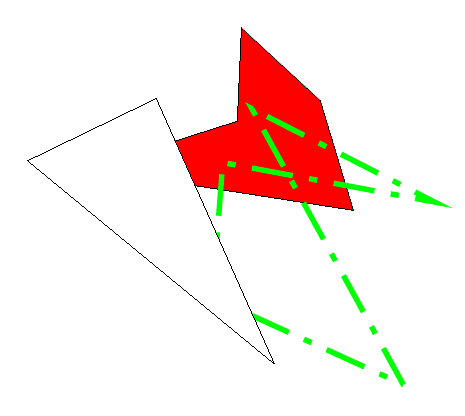
\begin{tikzpicture}
\pgftransformxscale{1.000000}
\pgftransformyscale{-1.000000}
\definecolor{dialinecolor}{rgb}{0.000000, 0.000000, 0.000000}
\pgfsetstrokecolor{dialinecolor}
\definecolor{dialinecolor}{rgb}{1.000000, 1.000000, 1.000000}
\pgfsetfillcolor{dialinecolor}
\pgfsetlinewidth{0.000000\du}
\pgfsetdash{}{0pt}
\pgfsetdash{}{0pt}
\pgfsetmiterjoin
\pgfsetbuttcap
\definecolor{dialinecolor}{rgb}{1.000000, 0.000000, 0.000000}
\pgfsetfillcolor{dialinecolor}
\fill (6.900000\du,5.650000\du)--(7.000000\du,3.400000\du)--(8.900000\du,5.150000\du)--(9.700000\du,7.800000\du)--(3.300000\du,6.800000\du)--cycle;
\definecolor{dialinecolor}{rgb}{0.000000, 0.000000, 0.000000}
\pgfsetstrokecolor{dialinecolor}
\draw (6.900000\du,5.650000\du)--(7.000000\du,3.400000\du)--(8.900000\du,5.150000\du)--(9.700000\du,7.800000\du)--(3.300000\du,6.800000\du)--cycle;
\pgfsetlinewidth{0.130000\du}
\pgfsetdash{{1.000000\du}{0.400000\du}{0.200000\du}{0.400000\du}}{0cm}
\pgfsetdash{{1.000000\du}{0.400000\du}{0.200000\du}{0.400000\du}}{0cm}
\pgfsetmiterjoin
\pgfsetbuttcap
\definecolor{dialinecolor}{rgb}{0.000000, 1.000000, 0.000000}
\pgfsetstrokecolor{dialinecolor}
\draw (10.900000\du,12.000000\du)--(7.250000\du,5.350000\du)--(11.650000\du,7.600000\du)--(11.650000\du,7.600000\du)--(6.550000\du,6.650000\du)--(6.300000\du,9.900000\du)--cycle;
\pgfsetlinewidth{0.000000\du}
\pgfsetdash{}{0pt}
\pgfsetdash{}{0pt}
\pgfsetmiterjoin
\pgfsetbuttcap
\definecolor{dialinecolor}{rgb}{1.000000, 1.000000, 1.000000}
\pgfsetfillcolor{dialinecolor}
\fill (1.850000\du,6.600000\du)--(4.950000\du,5.100000\du)--(7.800000\du,11.500000\du)--cycle;
\definecolor{dialinecolor}{rgb}{0.000000, 0.000000, 0.000000}
\pgfsetstrokecolor{dialinecolor}
\draw (1.850000\du,6.600000\du)--(4.950000\du,5.100000\du)--(7.800000\du,11.500000\du)--cycle;
\end{tikzpicture}
